% Draft v0.3 (2026-11-25).  Target: Physical Review E, Regular Article.
% Figures are read from ../figures (made by figures/fig*.py); nothing in this folder is edited by hand.
\documentclass[reprint,aps,pre,superscriptaddress,longbibliography,floatfix,amsmath,amssymb]{revtex4-2}
\usepackage{graphicx}
\usepackage{bm}
\usepackage[colorlinks=true,allcolors=blue]{hyperref}
\graphicspath{{../figures/}}

% --- notation: one place for every symbol ---
\newcommand{\Nst}{N^{*}}                 % melting length 2 log2(1/z)
\newcommand{\sig}{\sigma}                % uncompensated fraction (scaling limit)
\newcommand{\dst}{d^{*}}                 % frozen length, half edge = 1
\newcommand{\rM}{r_{M}}
\newcommand{\pM}{p_{M}}
\newcommand{\Qun}{Q_{\rm un}}
\newcommand{\dd}{\mathrm{d}}
\newcommand{\ee}{\mathrm{e}}
\newcommand{\ii}{\mathrm{i}}

\begin{document}

\title{Thermal vacancies melt arctic order: corner charges and an exact solution for the Aztec diamond}

% TODO(author list): only the corresponding author is entered.
\author{Changyeon Won}
\email{cywon@khu.ac.kr}
\affiliation{Department of Physics, Kyung Hee University, Seoul 02447, Republic of Korea}

\date{\today}

\begin{abstract}
Domino tilings of the Aztec diamond are frozen outside an inscribed circle because the boundary fixes the height field. We ask how this boundary-induced order responds to thermal vacancies, unpaired cells that appear with fugacity $z$ and carry a sublattice charge. The staircase edges of the diamond are charged plates that adsorb vacancies, and the only parameter in the scaling limit is $x=2\log_2(1/z)/N$, where $N$ is the order of the diamond. Because the number of adsorbed vacancies is fixed by the heights of the four corners, the fugacity enters the variational problem for the height field only through point sources of strength $x\ln 2$ at the corners, with free boundaries elsewhere. We solve this free-boundary problem for all $x$ by a hodograph transformation and express the solution through complete elliptic integrals. The frozen regions shrink to four separate corners whose size, $(4/\pi)\ln(1/z)$ lattice spacings for large diamonds, does not grow with $N$; arctic order therefore persists only up to sizes $N\simeq 2\log_2(1/z)$. The predicted fraction of uncompensated edge charge agrees with arbitrary-precision enumeration up to $N=192$ to between $10^{-6}$ and $10^{-4}$. Two uniform strip geometries with closed-form adsorption isotherms show that the type of frozen state decides whether melting has a threshold. For artificial spin ices described by dimer covers, the results give the size of ordered corners in terms of the defect energy and temperature.
\end{abstract}

\maketitle

%=====================================================================
\section{Introduction}\label{sec:intro}
%=====================================================================

In systems governed by a local conservation law, the shape of the boundary can determine the state of the bulk. Dimer coverings are the best understood example. A covering of a planar bipartite graph is encoded by a height function~\cite{TODO-thurston1990}, the boundary of the region fixes the height on its rim, and in the limit of a large region the height in the interior converges to the maximizer of an entropy functional~\cite{cohn2001}. For some regions the maximizer has frozen parts, where only one type of dimer occurs. The Aztec diamond of order $N$, which has $2^{N(N+1)/2}$ domino tilings~\cite{TODO-elkies1992}, is frozen outside the circle inscribed in it~\cite{TODO-jockusch1998,TODO-cohn1996}: the arctic circle. Such limit shapes are now understood in great generality through the complex Burgers equation~\cite{kenyon2007}.

This order exists only because every cell is covered. A real system at nonzero temperature has defects. In artificial spin ice~\cite{TODO-wang2006,TODO-nisoli2013}, several lattices have low-energy manifolds that map onto dimer covers, and their excitations are topologically charged defects of that cover~\cite{lao2018}. % TODO-shah2025: add the reference that motivated this work (arXiv:2506.15769) once its bibliographic data are confirmed.
In the dimer language the elementary defect is a vacancy (monomer), a cell that is not covered. A vacancy is a vortex of the height field and carries a charge $\pm 1$ given by its sublattice~\cite{TODO-fisher1963}. At a finite vacancy fugacity $z$ the vacancies form a two-component plasma that screens the Coulomb interaction~\cite{krauth2003,TODO-papanikolaou2007}. The question of this paper is what such a plasma does to boundary-induced order: how large must $z$ be, for a diamond of order $N$, to melt the frozen regions, and what replaces them?

The question has two parts, and existing results cover neither. The first part is how a boundary interacts with vacancies. For a straight boundary with monomers allowed on it, Berestycki, Lis, and Qian proved that the height field converges to the same Neumann free field for every positive boundary fugacity~\cite{berestycki2023}; the macroscopic state does not depend on $z$. Ciucu and coworkers found that gaps are repelled or attracted by a boundary according to whether it is constrained or free~\cite{ciucu2011,ciucu2014}. We show in Sec.~\ref{sec:model} that these boundaries are neutral, and that a second type, the staircase boundary, is charged. A charged boundary adsorbs vacancies in proportion to its length, and the adsorbed layer changes the boundary condition for the height field. All four edges of the Aztec diamond are of this type.

The second part is how the adsorbed vacancies change the limit shape. Limit shapes with defects placed on the boundary are known when the defect positions are prescribed: Ciucu and Krattenthaler obtained the exact weight of a pair of boundary dents of the Aztec diamond and its asymptotics~\cite{ciucu2023}, and Di~Francesco and Guitter found the arctic curve of Aztec rectangles for a prescribed density of defects along one side~\cite{difrancesco2019}. Limit shapes with free boundaries were obtained for lozenge tilings and for free-boundary Schur processes~\cite{difrancesco2012,betea2018}, in ensembles without a vacancy fugacity. Here the density of defects is not prescribed. It is selected thermodynamically by the fugacity, and it varies along the edge.

Our results are as follows. (i) The scaling variable is $x=\Nst/N$ with $\Nst=2\log_2(1/z)$; arctic order is intact for $x>1$ and melts for $x<1$. (ii) The number of vacancies adsorbed on an edge equals a difference of corner heights. The fugacity therefore enters the variational problem only as point sources of strength $x\ln 2$ at the four corners, and the edges become free boundaries (Sec.~\ref{sec:corner}). (iii) After a hodograph transformation the free-boundary problem becomes a linear problem in a fixed sector, which we solve for all $x$ (Sec.~\ref{sec:exact}). The solution gives the fraction $\sig(x)$ of edge charge that remains uncompensated, the vacancy density along the edge, and the boundary of the frozen regions. (iv) The frozen regions are four disconnected corners. For $x\to 0$ each has a size of $(4/\pi)\ln(1/z)$ lattice spacings, independent of $N$. (v) Two uniform strip geometries have closed-form isotherms, one with a threshold and one without, and explain the two limits of the Aztec result (Sec.~\ref{sec:uniform}). The derivation of (ii)--(iv) rests on a variational principle that we argue for but do not prove; the outcome is tested against exact enumeration in Sec.~\ref{sec:tests}. Section~\ref{sec:discussion} discusses the meaning of the results and their range of validity.

%=====================================================================
\section{Model and symmetries}\label{sec:model}
%=====================================================================

\subsection{Dimers with vacancies}

We consider a region $A$ of the square lattice, made of unit cells colored as a checkerboard. A configuration is a set of dominoes, each covering two adjacent cells, such that no cell is covered twice; the uncovered cells are vacancies [Fig.~\ref{fig:model}(a)]. Each vacancy has weight $z$,
\begin{equation}\label{eq:Z}
  Z_A(z)=\sum_{V}z^{|V|}\,M(A\setminus V),
\end{equation}
where the sum runs over sets $V$ of cells and $M(A\setminus V)$ is the number of domino tilings of the remaining cells. In a physical realization $z=\ee^{-E_d/k_BT}$, with $E_d$ the energy of a defect. We use two versions of the model. In the \emph{full model} $V$ is any set of cells. In the \emph{boundary model} $V$ is restricted to the outermost cells of the region, which makes Eq.~\eqref{eq:Z} a Pfaffian~\cite{giuliani2016} and allows enumeration at large sizes. Section~\ref{sec:tests} argues, and tests numerically, that the two versions have the same scaling limit on the Aztec diamond.

\subsection{Charge and height}

A vacancy on an even (odd) cell carries charge $+1$ ($-1$). Because every domino covers one cell of each color, the total charge $n_+-n_-$ of any configuration equals the color imbalance of the region; it is zero for the regions considered here. In terms of Thurston's height function~\cite{TODO-thurston1990}, which is defined on the vertices and changes by $\pm1$ along cell sides not crossed by a domino, a vacancy is a vortex around which the height winds by $\pm4$. The effective description is a Coulomb gas: vacancies of opposite charge attract and those of equal charge repel logarithmically, and a charge-$q$ vacancy has scaling dimension $q^2/4$, in agreement with the exponent $1/2$ of the monomer-monomer correlation~\cite{TODO-fisher1963}. The bulk properties of the resulting plasma are summarized in Appendix~\ref{app:bulk}.

\subsection{Neutral and charged boundaries}

The cells along a boundary are the ones that can lose their partner to the outside, so the color pattern of the boundary cells determines how the boundary couples to the charge. Two cases follow from symmetry alone [Fig.~\ref{fig:model}(b)].

Along a straight edge, the unit translation parallel to the edge exchanges the two colors. It maps the model onto itself with all charges reversed, so the edge carries no line charge. A straight edge is neutral. It neither adsorbs nor repels a net charge, and it interacts with a vacancy only through an image (Appendix~\ref{app:bulk}).

Along a staircase edge, the diagonal translation preserves the colors, and all outermost cells have the same color. Removing one of them lowers the boundary height by 4 relative to the unperturbed staircase. A staircase edge is therefore a charged plate: in the height language it imposes the maximal slope, and each vacancy adsorbed on it reduces that slope. If $\rho$ is the density of vacancies per edge cell, the boundary slope is reduced by the factor
\begin{equation}\label{eq:slope}
  h=1-2\rho ,
\end{equation}
so that $\rho=1/2$ corresponds to a flat boundary. By Gauss's law a staircase edge facing a neutral bulk of vacancy density $n$ adsorbs a charge $(1-n)/2$ per edge cell, which we confirmed by transfer matrices (Appendix~\ref{app:bulk}).

\begin{figure*}[t]
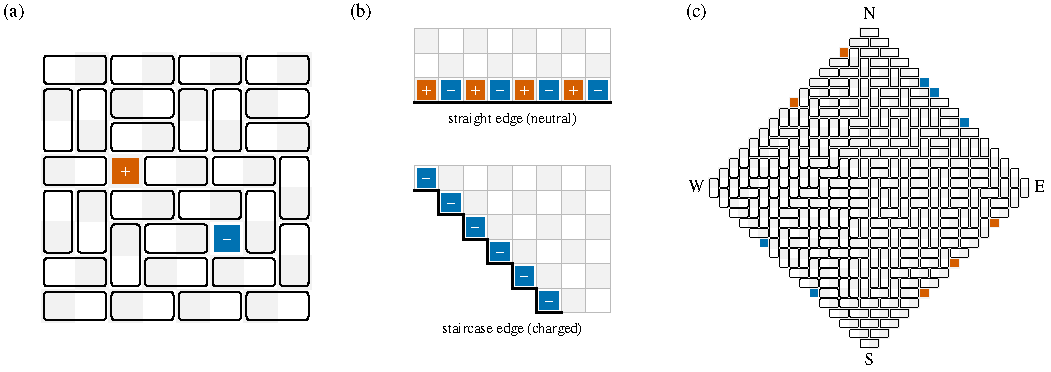
\includegraphics[width=\textwidth]{fig1_model.pdf}
\caption{Vacancies are sublattice charges, and staircase edges are charged. (a) A domino configuration with one vacancy on each sublattice (charges $+$ and $-$). (b) Outermost cells of a straight edge alternate in color, so the edge is neutral; those of a staircase edge have one color, so the edge is charged. (c) Equilibrium configuration of the Aztec diamond of order $N=16$ at $z=1/16$ ($x=0.5$) in the boundary model. Vacancies (colored by sublattice) are adsorbed near the middle of the edges, and the brick patterns of the frozen state survive only near the corners S, E, N, and W. The sample was drawn with the sampler described in Appendix~\ref{app:numerics}.}
\label{fig:model}
\end{figure*}

\subsection{Aztec diamond and the scaling variable}

The Aztec diamond of order $N$ consists of the cells whose centers satisfy $|X|+|Y|\le N$ [Fig.~\ref{fig:model}(c)]. Its four edges are staircases with $N$ outermost cells each. The rotation by $90^\circ$ exchanges the colors, so the symmetry group is generated by this rotation combined with charge conjugation and by the diagonal reflections, which preserve colors. Consequently the two edges meeting at the corners S and N carry vacancies of one sign, the other two edges carry the opposite sign, all four edges have the same vacancy density profile, and the profile is symmetric about the middle of the edge.

The competition that controls melting can be read off from a single pair of vacancies. Removing the two cells at the middle of two adjacent edges multiplies the number of tilings by a factor that grows as $2^N/(\pi N)$~\cite{ciucu2023}, whereas the pair costs $z^2$. With
\begin{equation}\label{eq:x}
  \Nst=2\log_2(1/z),\qquad x=\frac{\Nst}{N},
\end{equation}
the weight of the pair is $2^{N(1-x)}$ up to a power of $N$. For $x>1$ adsorbed pairs are exponentially rare and the arctic circle is intact; for $x<1$ they proliferate. The length $\Nst$ is the size above which arctic order melts. It depends on the fugacity only logarithmically and is much shorter than the bulk screening length, which grows as $z^{-4/7}$ (Appendix~\ref{app:bulk}). The scaling limit of this paper is $N\to\infty$ at fixed $x$.

We characterize the adsorbed layer by its mean density $\bar\rho$ per edge cell and by the fraction of edge charge that is not compensated,
\begin{equation}\label{eq:sigma}
  \sig=1-2\bar\rho .
\end{equation}
The intact diamond has $\sig=1$, and a diamond whose edges have become flat on average has $\sig=0$.

%=====================================================================
\section{Uniform geometries}\label{sec:uniform}
%=====================================================================

Before turning to the diamond we solve two strips in which charged edges of opposite sign face each other and the state is uniform along the strip. Vacancies then appear in pairs, one on each edge, and the height is linear across the strip, so the variational problem reduces to maximizing a function of the single density $\rho$.

\subsection{Staircase strip of dominoes}

Consider a strip bounded by two parallel staircase edges with $W$ cells on each lattice diagonal, and vacancies allowed on the outermost cells of both edges. Without vacancies the strip is frozen, with zero entropy per cell: two types of domino alternate in layers. With vacancy density $\rho$ on each edge the slope across the strip is $1-2\rho$ and the entropy per cell follows from the entropy function of domino tilings~\cite{cohn2001} as $e(\rho)/2$ with
\begin{equation}
  e(\rho)=\frac{2}{\pi}\left[L\!\left(\frac{\pi(1-\rho)}{2}\right)+L\!\left(\frac{\pi\rho}{2}\right)\right],
\end{equation}
where $L(\theta)=-\int_0^\theta\ln(2\sin t)\,\dd t$ is the Lobachevsky function. Since $e'(\rho)=\ln\cot(\pi\rho/2)$, balancing the entropy gained in a strip of width $W$ against the cost of a vacancy pair gives $e'(\rho)=(2/W)\ln(1/z)$, that is,
\begin{equation}\label{eq:strip}
  \rho=\frac{2}{\pi}\arctan\!\left(z^{2/W}\right).
\end{equation}
The isotherm has no threshold: the density is positive for every $z>0$ and reaches the flat value $1/2$ at $z=1$. The reason is the term $-\rho\ln\rho$ in $e(\rho)$ at small $\rho$, which makes the first vacancies infinitely favorable per unit length. Figure~\ref{fig:iso}(a) compares Eq.~\eqref{eq:strip} with exact transfer-matrix results.

\subsection{Lozenge capacitor}

The second strip is made of lozenges. Take $N$ layers of a single type of lozenge between two edges of opposite charge. A pair of vacancies, one on each edge, is connected by a lattice path that advances by $0$ or $+1$ in each layer, and the paths of different pairs do not intersect. For a density $\rho$ of paths per edge cell the entropy per cell is
\begin{equation}
  s_{\rm loz}(\rho)=\frac{1}{\pi}\left[2L\!\left(\frac{\pi\rho}{2}\right)+L\bigl(\pi(1-\rho)\bigr)\right],
\end{equation}
with $s_{\rm loz}'(\rho)=\ln[2\cos(\pi\rho/2)]$. A path of $N$ layers costs $z^2$, so that $s_{\rm loz}'(\rho)=x\ln 2$ with $x$ defined as in Eq.~\eqref{eq:x}, and
\begin{equation}\label{eq:loz}
  \rho=\frac{2}{\pi}\arccos\!\left(2^{x-1}\right)\quad(x<1),\qquad \rho=0\quad(x\ge1).
\end{equation}
Here melting has a threshold at $x=1$, and the density grows as $(1-x)^{1/2}$ beyond it, as at a commensurate-incommensurate transition~\cite{TODO-pokrovsky1979}. Each path has at most two choices per layer, so its entropy cannot exceed $N\ln 2$, and a pair is favorable only if $z^2 2^N>1$. Figure~\ref{fig:iso}(b) compares the free energy $s_{\rm loz}(\rho)-\rho\,x\ln2$ evaluated at Eq.~\eqref{eq:loz} with exact transfer matrices.

\begin{figure*}[t]
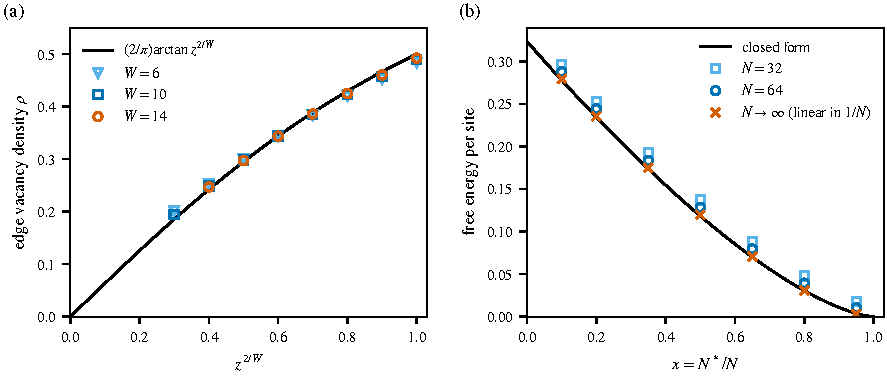
\includegraphics[width=0.86\textwidth]{fig2_isotherms.pdf}
\caption{Closed-form adsorption isotherms of two uniform strips agree with exact transfer matrices. (a) Staircase strip of dominoes: vacancy density on the edge cells against $z^{2/W}$ for strips with $W$ cells per diagonal (symbols), and Eq.~\eqref{eq:strip} (line). There is no threshold. (b) Lozenge capacitor: free energy per cell against $x$ for $N=32$ and $64$ layers on a ring of 12 cells, their extrapolation linear in $1/N$ (crosses), and the closed form from Eq.~\eqref{eq:loz} (line). Melting starts at $x=1$. The transfer-matrix values are exact to numerical precision.}
\label{fig:iso}
\end{figure*}

\subsection{What decides the threshold}

The two strips differ in the position of the frozen slope on the boundary of the set of allowed slopes. In the lozenge capacitor the frozen state has a single type of tile and its slope is a vertex of the slope polygon; defects are directed paths with bounded entropy, and melting has a threshold. In the staircase strip the frozen slope lies in the interior of a side of the polygon, the frozen state mixes two types of tile, and the entropy of defects is unbounded per unit length. Along an edge of the Aztec diamond the slope sweeps a whole side of the polygon, from a vertex at each corner to the midpoint of the side at the middle of the edge. The diamond therefore combines the two behaviors: a threshold at $x=1$, governed by the vertex-type state that would have to be created at the middle of the edge, and corners that remain frozen for all $x>0$. Neither isotherm describes the diamond quantitatively, because adjacent edges are coupled through the interior: the vacancy density at the middle of an edge of the diamond (Table~\ref{tab:sol}) is not reproduced by Eq.~\eqref{eq:strip} with $z^{2/W}$ replaced by $2^{-ax}$ for any single constant $a$.

%=====================================================================
\section{Aztec diamond: corner charges}\label{sec:corner}
%=====================================================================

\subsection{Variational principle}

We use coordinates $(u,v)$ along the two edges that meet at the corner S, scaled so that the diamond is the square $D=[0,2]^2$ and half an edge has unit length; S is at $(0,0)$, the middle of the edge SE at M$\,=(1,0)$, and the center at O$\,=(1,1)$. The macroscopic height $H(u,v)$ is normalized so that $|\partial_uH|\le1$ along the edges, with equality on a vacancy-free staircase. For a fixed set of boundary vacancies the remaining region is simply connected with a prescribed boundary height, and the number of its tilings is given by the variational principle of Cohn, Kenyon, and Propp~\cite{cohn2001}. Summing over vacancy sets adds only an entropy of order $N$ and a factor $z^{|V|}$, which leads to
\begin{multline}\label{eq:var0}
  \lim_{N\to\infty}\frac{\ln Z}{N^2}=\max_{H}\biggl[\frac12\int_D s(\nabla H)\,\dd u\,\dd v\\
  -\frac{x\ln2}{2}\sum_{\rm edges}\int_0^2\rho\,\dd\ell\biggr],
\end{multline}
where $s$ is the entropy per cell of domino tilings with slope $\nabla H$~\cite{cohn2001}, $\rho$ is the vacancy density on the edge, related to the tangential slope by Eq.~\eqref{eq:slope}, and the maximum is over all $H$ whose slope is admissible. The boundary values of $H$ are free. Appendix~\ref{app:variational} gives the argument for Eq.~\eqref{eq:var0} and states what remains to be proved.

\subsection{The fugacity as corner sources}

By Eq.~\eqref{eq:slope} the number of vacancies on an edge is a boundary term: $\int_0^2\rho\,\dd\ell=1-\Delta H/2$, where $\Delta H$ is the height difference between the two ends of the edge. The height alternately rises and falls on consecutive edges, so the sum over edges collects each corner twice, and Eq.~\eqref{eq:var0} becomes, up to a constant,
\begin{multline}\label{eq:var}
  \Phi[H]=\frac12\int_D s(\nabla H)\,\dd u\,\dd v\\
  +\frac{x\ln2}{4}\bigl[H({\rm S})+H({\rm N})-H({\rm W})-H({\rm E})\bigr].
\end{multline}
This is the central step. Thermal vacancies act on the height field as four point sources at the corners, of alternating sign and of strength proportional to $x$. Nothing else in the problem depends on the fugacity.

The stationarity conditions of Eq.~\eqref{eq:var} are the Euler-Lagrange equation $\nabla\!\cdot\!\bm{j}=0$ for the current $\bm j=\partial s/\partial\nabla H$ in the interior, and the natural boundary condition $\bm j\cdot\bm n=0$ on every part of an edge that carries vacancies. Where the constraint $\rho\ge0$ is active the slope is maximal and the state is frozen. The fraction defined in Eq.~\eqref{eq:sigma} is the height of a corner above the middle of the edge,
\begin{equation}\label{eq:sigH}
  \sig=H({\rm S})-H({\rm M}).
\end{equation}

Because the edges obey the natural boundary condition, the solution can be continued by reflection across them, as for free-boundary lozenge tilings~\cite{difrancesco2012}. The reflected problem lives on the whole plane and has point charges of strength $q=x\ln2$ and alternating sign on the square lattice of corner images [Fig.~\ref{fig:corner}(a) and \ref{fig:corner}(b)]. Around each charge the slope saturates and a frozen region forms; between them the tiling is liquid. The Aztec diamond is one unit cell of this checkerboard.

\begin{figure*}[t]
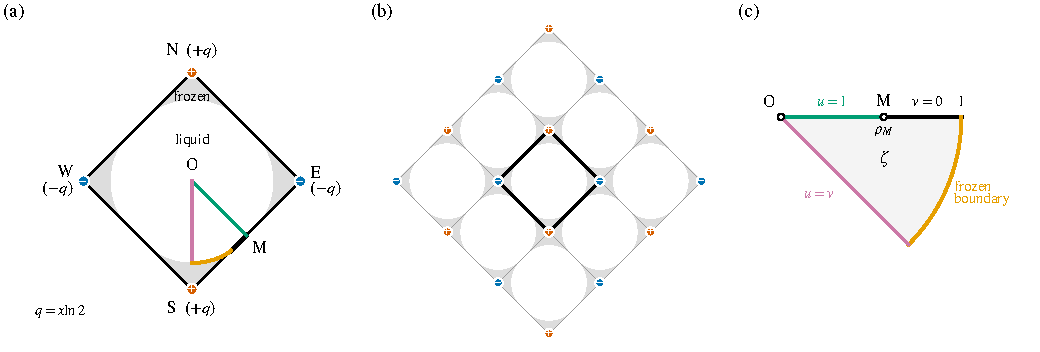
\includegraphics[width=\textwidth]{fig3_corner_charges.pdf}
\caption{The fugacity acts as point charges at the corners, and the hodograph transformation maps the liquid region onto a fixed sector. (a) Aztec diamond in the scaling limit at $x=0.8$, with charges $\pm q$, $q=x\ln2$, at the corners and the frozen corners (gray) of the exact solution. The fundamental triangle S--M--O is bounded by the vacancy-bearing part of the edge (black), the symmetry axis MO (green), the diagonal (purple), and the frozen boundary (orange). (b) Reflection across the edges gives a checkerboard of point charges in the plane; the diamond is one cell. (c) Image of the liquid part of the triangle in the plane of $\zeta$, Eq.~\eqref{eq:zeta}: the sector $|\zeta|<1$, $-\pi/4<\arg\zeta<0$, for every $x$. The parameter $x$ enters only through the position $r_M$ of the point M.}
\label{fig:corner}
\end{figure*}

\subsection{An isolated frozen corner}

For small $x$ the frozen regions are small and far apart, and each can be treated in isolation. Near the flat state the entropy is
\begin{equation}\label{eq:stiff}
  s(\nabla H)\simeq\frac{G}{\pi}-\frac{\pi}{16}|\nabla H|^2 ,
\end{equation}
with $G$ Catalan's constant, so that far from a corner of charge $q$ the height is harmonic, $H\simeq-(8q/\pi^2)\ln r$. Close to the corner the full nonlinear problem must be solved. The solution of the complex Burgers equation~\cite{kenyon2007} that has this far field and the two reflection symmetries of a corner is
\begin{equation}\label{eq:island}
  (1-\omega^2)\,v-2\omega\,u=\dst\,\frac{2\omega(1-\omega^2)}{1+\omega^2},\qquad \dst=\frac{4}{\pi}\,x\ln2 ,
\end{equation}
where $\omega(u,v)$ is the complex slope variable defined in Sec.~\ref{sec:exact}. The corner is frozen along each edge up to the distance $\dst$, and beyond it the vacancy density is
\begin{equation}\label{eq:rhoiso}
  \rho(d)=\frac1\pi\arccos\frac{\dst}{d}\qquad(d>\dst),
\end{equation}
which starts as a square root at the end of the frozen segment. In lattice units $\dst$ corresponds to
\begin{equation}\label{eq:ell}
  \ell=\frac{N}{2}\,\dst=\frac{4}{\pi}\ln\frac1z
\end{equation}
cells. The size of a frozen corner is set by the fugacity alone. It does not grow with the system, in contrast to the frozen regions of the intact diamond, which occupy a fixed fraction of the area.

\subsection{Small-$x$ law}

The height of a corner follows from Eq.~\eqref{eq:island}, which gives $H(0)-H(r)\simeq(2\dst/\pi)\ln(2\ee\,r/\dst)$ at distances $r\gg\dst$, and from the logarithmic potential of all other charges of the checkerboard. The alternating lattice sum is
\begin{equation}
  \sideset{}{'}\sum_{a,b}(-1)^{a+b}\ln\sqrt{a^2+b^2}=\ln\frac{\Gamma(1/4)^2}{4\sqrt\pi},
\end{equation}
which we evaluated numerically and identified with this closed form. With Eq.~\eqref{eq:sigH} the result is
\begin{equation}\label{eq:smallx}
  \sig(x)\simeq\frac{8\ln2}{\pi^2}\,x\ln\frac{B}{x},\qquad B=\frac{4\pi^{3/2}\ee}{\Gamma(1/4)^2\ln2}\approx6.645 .
\end{equation}
Each factor has a direct meaning. The strength $x\ln2$ is the cost of a vacancy pair measured against the entropy $N\ln2$ that a pair can gain; the prefactor $8/\pi^2$ is the inverse stiffness of the height field, Eq.~\eqref{eq:stiff}; and the logarithm is the potential of a point charge in two dimensions, cut off at the size $\dst$ of the frozen corner and at the distance to the neighboring charges. Multiplying by the number of edge cells, the uncompensated charge of an edge is
\begin{equation}\label{eq:Qun}
  \Qun\simeq\frac{4\ln2}{\pi^2}\,\Nst\ln\frac{BN}{\Nst}\qquad(N\gg\Nst),
\end{equation}
which grows only logarithmically with the size of the diamond: almost all of the edge charge is compensated by adsorbed vacancies.

%=====================================================================
\section{Exact solution}\label{sec:exact}
%=====================================================================

\subsection{Hodograph plane}

For domino tilings the current $\bm j$ and the slope are parametrized by a complex number $\omega$ in the upper half plane, with $(\partial s/\partial H_u,\partial s/\partial H_v)=\mp\tfrac14(\ln|\omega|,\ln|\eta|)$ and $1+\omega+\eta-\omega\eta=0$, and the Euler-Lagrange equation is equivalent to the statement that $\omega(u,v)$ satisfies~\cite{kenyon2007}
\begin{equation}\label{eq:burgers}
  v-\lambda(\omega)\,u=\Psi(\omega),\qquad \lambda(\omega)=\frac{2\omega}{1-\omega^2},
\end{equation}
with an analytic function $\Psi$. Read as an equation for $(u,v)$ at given $\omega$, Eq.~\eqref{eq:burgers} is linear in $\Psi$. This is the hodograph point of view: the symmetry lines and the vacancy-bearing edge, whose positions in the $(u,v)$ plane are unknown, are fixed curves in the plane of $\omega$. With
\begin{equation}\label{eq:zeta}
  \zeta=\frac{\omega-\ii}{\omega+\ii}
\end{equation}
the liquid part of the fundamental triangle S--M--O is mapped, for every $x$, onto the sector $|\zeta|<1$, $-\pi/4<\arg\zeta<0$ [Fig.~\ref{fig:corner}(c)]. The center O is at $\zeta=0$. On the real side, $\zeta=r$, the segment $0<r<\rM$ is the symmetry axis MO, where $u=1$, and the segment $\rM<r<1$ is the vacancy-bearing part of the edge, where $v=0$ and the tangential slope is
\begin{equation}\label{eq:hr}
  h=\frac4\pi\arctan r ,\qquad \rho=\frac12-\frac2\pi\arctan r .
\end{equation}
The ray $\arg\zeta=-\pi/4$ is the diagonal SO, where $u=v$, and the arc $|\zeta|=1$ is the boundary of the frozen corner. The variable $J=(\zeta^4+\zeta^{-4})/2$ opens the sector to a half plane, where the boundary conditions define a Riemann-Hilbert problem with piecewise constant coefficients. Requiring $\Psi$ to be finite everywhere selects one solution, which depends on the single parameter $\rM\in(0,1)$. Appendix~\ref{app:rh} gives the solution as a rapidly convergent series; here we state it in closed form.

\subsection{Solution}

Let $\pM=\rM^2+\rM^{-2}$, $k^2=(\pM-2)/(2\pM)$, and $P=r^2+r^{-2}$, and define
\begin{equation}\label{eq:I}
  I(P)=\sqrt{\frac{2}{\pM}}\left[\frac{\Pi(n_1,k)}{\pM-P}+\frac{\Pi(n_2,k)}{\pM+P}\right],
\end{equation}
with $n_{1}=(\pM-2)/(\pM-P)$ and $n_{2}=(\pM-2)/(\pM+P)$,
where $\Pi(n,k)=\int_0^{\pi/2}\dd\theta\,(1-n\sin^2\theta)^{-1}(1-k^2\sin^2\theta)^{-1/2}$ is the complete elliptic integral of the third kind, taken as a principal value, $\Pi(n,k)=K(k)-\Pi(k^2/n,k)$, when $n>1$. On the vacancy-bearing part of the edge ($\rM<r<1$) the distance from the corner is
\begin{equation}\label{eq:u}
  u(r)=1-\frac1\pi\sqrt{(P+2)(\pM^2-P^2)}\;I(P),
\end{equation}
which with Eq.~\eqref{eq:hr} gives the vacancy density profile $\rho(u)$ in parametric form. On the symmetry axis ($0<r<\rM$),
\begin{equation}\label{eq:v}
  v(r)=1+\frac1\pi\sqrt{(P-2)(P^2-\pM^2)}\;I(P).
\end{equation}
The frozen length is $\dst=u(r\to1)$,
\begin{multline}\label{eq:dstar}
  \dst=1-\frac{2}{\pi}\sqrt{\frac{2(\pM^2-4)}{\pM}}\\
  \times\left[\frac{K-E/(1-k^2)}{\pM-2}+\frac{\Pi(\kappa,k)}{\pM+2}\right],
\end{multline}
with $\kappa=(\pM-2)/(\pM+2)$ and $K$ and $E$ the complete elliptic integrals of the first and second kind. The parameter $\rM$ is related to $x$ by conservation of the current emitted by the corner source,
\begin{equation}\label{eq:xcond}
  x\ln2=\int_0^{\rM}v(r)\,\frac{2\,\dd r}{1-r^2},
\end{equation}
and the uncompensated fraction is
\begin{equation}\label{eq:sigexact}
  \sig=h_M+\int_{h_M}^{1}u\,\dd h,\qquad h_M=\frac4\pi\arctan\rM .
\end{equation}
The density profile and the frozen length are thus given by complete elliptic integrals, while $x$ and $\sig$ require one further quadrature each; we have not been able to reduce these two to elliptic integrals. Table~\ref{tab:sol} lists representative values and Fig.~\ref{fig:sigma}(a) shows $\sig(x)$.

\begin{table}[b]
\caption{Exact solution in the scaling limit: hodograph parameter $\rM$, uncompensated fraction $\sig$, frozen length $\dst$ in units of half an edge, and vacancy density $\rho_M$ at the middle of the edge, from Eqs.~\eqref{eq:hr}--\eqref{eq:sigexact}.}
\label{tab:sol}
\begin{ruledtabular}
\begin{tabular}{ccccc}
$x$ & $\rM$ & $\sig$ & $\dst$ & $\rho_M$\\ \hline
0.05 & 0.02894 & 0.137354 & 0.04413 & 0.4816\\
0.1 & 0.05799 & 0.235729 & 0.08825 & 0.4631\\
0.2 & 0.11685 & 0.393292 & 0.17651 & 0.4259\\
0.3 & 0.17753 & 0.520891 & 0.26481 & 0.3881\\
0.4 & 0.24117 & 0.628520 & 0.35324 & 0.3493\\
0.5 & 0.30927 & 0.720715 & 0.44202 & 0.3091\\
0.6 & 0.38397 & 0.799931 & 0.53158 & 0.2666\\
0.7 & 0.46871 & 0.867527 & 0.62286 & 0.2210\\
0.8 & 0.56982 & 0.924080 & 0.71797 & 0.1703\\
0.9 & 0.70261 & 0.969303 & 0.82293 & 0.1101\\
\end{tabular}
\end{ruledtabular}
\end{table}

\subsection{Limits}

For $\rM\to1$ the solution gives $x\to1$, $\sig\to1$, and $\dst\to1$, and the frozen boundary becomes the arctic circle. The threshold $x=1$ of Sec.~\ref{sec:model} is recovered, and the integral in Eq.~\eqref{eq:xcond} tends to $\ln2$, which is an independent check of the normalization. Close to the threshold the vacancies occupy a short interval of half-width $w$ around the middle of the edge with a semicircular density, and $1-\sig=w^2$. Numerically the solution approaches
\begin{equation}\label{eq:near1}
  1-\sig=\frac{2\ln2\,(1-x)}{1-4\ln2+\ln[16/(1-\sig)]},
\end{equation}
the equilibrium condition of a one-dimensional gas of vacancies with logarithmic repulsion; the ratio of the two sides is between $0.9994$ and $1.0002$ for $3\times10^{-5}\le1-x\le1.5\times10^{-2}$. The onset is therefore linear in $1-x$ with a logarithmic correction, softer than the square root of the uniform capacitor, Eq.~\eqref{eq:loz}, because the vacancies first appear in a region whose width itself vanishes at the threshold.

For $\rM\to0$ the solution reduces to the isolated corner of Sec.~\ref{sec:corner}. We find $x\ln2\simeq(\pi/\varpi_{\rm L})\,\rM$ with the lemniscate constant $\varpi_{\rm L}=\Gamma(1/4)^2/(2\sqrt{2\pi})$, $\dst\simeq(4\ln2/\pi)\,x$, and Eq.~\eqref{eq:smallx} with a correction $-0.046\,x^3$ whose coefficient we determined only numerically. The small-$x$ law is accurate to $10^{-3}$ up to $x\approx0.3$ [Fig.~\ref{fig:sigma}(a)].

\begin{figure*}[t]
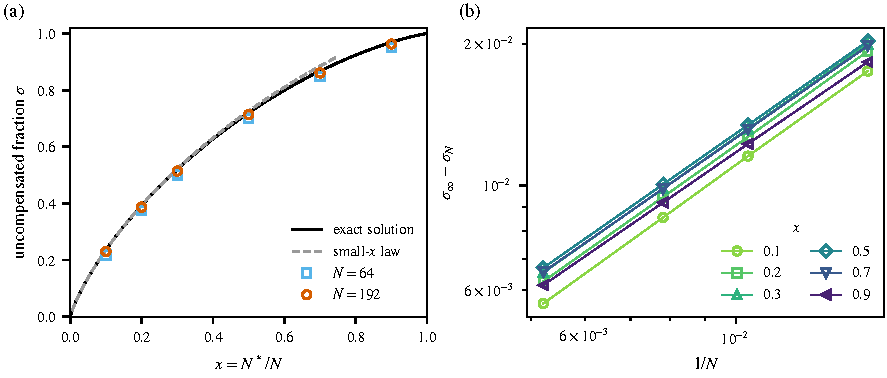
\includegraphics[width=0.86\textwidth]{fig4_sigma.pdf}
\caption{The exact solution for the uncompensated fraction agrees with enumeration without adjustable parameters. (a) $\sig(x)$ from Eq.~\eqref{eq:sigexact} (line), the small-$x$ law, Eq.~\eqref{eq:smallx} (dashed), and exact values of the boundary model at $N=64$ and $N=192$ (symbols). (b) Difference between the solution and the exact finite-size values $\sig_N$ for $N=64$, 96, 128, and 192, which decreases in proportion to $1/N$. The enumeration is exact, so the symbols have no error bars.}
\label{fig:sigma}
\end{figure*}

\subsection{Vacancy profile and frozen corners}

Figure~\ref{fig:profile} shows the vacancy density along an edge. The density vanishes as a square root at the ends of the frozen segments and is nearly constant in the middle; as $x$ decreases the frozen segments shorten and the plateau approaches the flat value $1/2$.

On the arc $|\zeta|=1$ the function $\Psi$ is real, and Eq.~\eqref{eq:burgers} describes a family of straight lines, $v+Tu=\Psi(T)$ with $T=\tan|\arg\zeta|$, whose envelope is the boundary of the frozen corner (Appendix~\ref{app:rh}). Figure~\ref{fig:frozen}(a) shows these boundaries. At $x=1$ they form the arctic circle, where the four frozen regions touch at the middle of the edges. For $x<1$ the regions detach from each other and retreat into the corners. Their extent along the edge, $\dst(x)$, is close to the isolated-corner value $(4\ln2/\pi)x$ up to $x\approx0.7$ and bends up to $1$ at the threshold [Fig.~\ref{fig:frozen}(b)].

\begin{figure}[t]
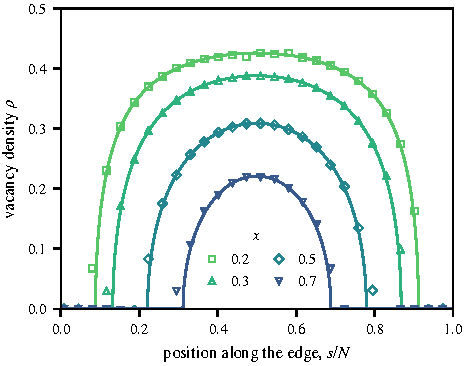
\includegraphics[width=\columnwidth]{fig5_profiles.pdf}
\caption{The vacancy density along an edge is flat in the middle and vanishes as a square root at the frozen corners. Lines: exact solution, Eqs.~\eqref{eq:hr} and \eqref{eq:u}. Symbols: exact densities of the boundary model at $N=40$ and $56$, extrapolated linearly in $1/N$ at fixed position $s/N$; every second point is shown.}
\label{fig:profile}
\end{figure}

\begin{figure*}[t]
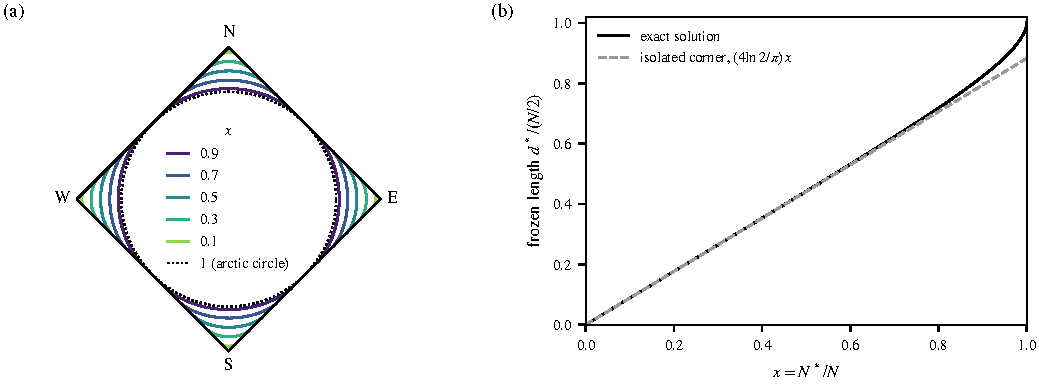
\includegraphics[width=\textwidth]{fig6_frozen.pdf}
\caption{Thermal vacancies shrink the frozen regions to four separate corners. (a) Boundaries of the frozen corners from the exact solution for several $x$; at $x=1$ they form the arctic circle (dotted). (b) Extent $\dst$ of a frozen corner along the edge, in units of half an edge, from Eq.~\eqref{eq:dstar} (line) and for an isolated corner, Eq.~\eqref{eq:island} (dashed).}
\label{fig:frozen}
\end{figure*}

%=====================================================================
\section{Tests}\label{sec:tests}
%=====================================================================

\subsection{Exact enumeration of the boundary model}

The partition function of the boundary model is a Pfaffian~\cite{giuliani2016}, and for the Aztec diamond the entries of the relevant matrix are known in closed form~\cite{ciucu2023} (Appendix~\ref{app:pfaffian}). The matrix can therefore be built from rational numbers and its determinant evaluated in arbitrary-precision arithmetic, which gives $\sig_N(x)=1-2\bar\rho$ exactly for any $N$; the limit on the size is memory. We computed $N\le192$.

Figure~\ref{fig:sigma}(b) shows that $\sig_N$ approaches the solution with a correction proportional to $1/N$. Extrapolating the values at $N=96$, 128, and 192 with a quadratic polynomial in $1/N$ gives the limits listed in Table~\ref{tab:check}. They agree with Eq.~\eqref{eq:sigexact} to within $4\times10^{-7}$ at $x=0.5$ and to within $7\times10^{-5}$ in the worst case, $x=0.1$. The larger differences at the two ends of the range occur where either the frozen corner or the vacancy-bearing interval spans few lattice cells at these sizes, so that the extrapolation is less accurate there; we have not quantified this. The density profiles agree point by point (Fig.~\ref{fig:profile}).

\begin{table}[b]
\caption{Uncompensated fraction in the scaling limit: extrapolation of exact boundary-model values ($N=96$, 128, 192; quadratic in $1/N$) against the solution of Sec.~\ref{sec:exact}.}
\label{tab:check}
\begin{ruledtabular}
\begin{tabular}{cccc}
$x$ & Enumeration & Solution & Difference\\ \hline
0.1 & 0.235796 & 0.235729 & $7\times10^{-5}$\\
0.2 & 0.393295 & 0.393292 & $3\times10^{-6}$\\
0.3 & 0.520893 & 0.520891 & $2\times10^{-6}$\\
0.5 & 0.720715 & 0.720715 & $4\times10^{-7}$\\
0.7 & 0.867520 & 0.867527 & $7\times10^{-6}$\\
0.9 & 0.969266 & 0.969303 & $4\times10^{-5}$\\
\end{tabular}
\end{ruledtabular}
\end{table}

\subsection{Optimality conditions}

The derivation in Sec.~\ref{sec:exact} assumed that the liquid region is mapped one-to-one onto the sector and that the solution without singularities is the relevant one. These assumptions can be replaced by a check of the result. The functional $\Phi$ of Eq.~\eqref{eq:var} is concave, and strictly concave on liquid slopes, so a height function that satisfies the optimality conditions is the maximizer. We verified numerically, at $x=0.2$, 0.5, and 0.8 and at 108 interior points of the sector, that the slope field obtained from Eq.~\eqref{eq:burgers} is a gradient and satisfies the Euler-Lagrange equation, with relative residuals between $10^{-8}$ and $4\times10^{-6}$, which is the accuracy of the finite differences used. The slopes were computed from the entropy function itself, so the check does not depend on sign conventions for $\omega$. The Jacobian of the map from $\zeta$ to $(u,v)$ has one sign and the image lies inside the triangle S--M--O. On the boundary the solution satisfies $v=0$ with vanishing normal current on the edge, $u=1$ on the symmetry axis, and $u=v$ on the diagonal, and its slope tends to the frozen value on the arc and to zero at the center.

Two steps are missing from a proof. Inside the frozen corners one must exhibit a divergence-free current that carries the corner source and stays within the bounds allowed for the frozen slope; this is the standard structure of frozen regions~\cite{kenyon2007}, but we have not constructed it. The second step concerns Eq.~\eqref{eq:var0} itself and is discussed in Appendix~\ref{app:variational}.

\subsection{Vacancies on all cells}

In the full model vacancies also enter the interior. At fixed $x$ their number is of order $N^2z^{8/7}=N^2\,2^{-4xN/7}$ (Appendix~\ref{app:bulk}) and vanishes in the scaling limit, so the interior of a large diamond is free of vacancies. What differs from the boundary model is the layer next to the edge, where an adsorbed vacancy of the full model can sit a few cells inside.

We argue that this difference is a boundary free energy. On a vacancy-bearing part of an edge the normal current vanishes and the tangential slope is $1-2\rho$, which is the uniform state of the staircase strip of Sec.~\ref{sec:uniform} at the same density. A vacancy displaced by $d$ cells from the edge is suppressed by a factor $\tan^d(\pi\rho/2)$ in that state, so the layer has a finite thickness. To first order the two partition functions then differ by a local term,
\begin{equation}\label{eq:dg}
  \ln Z_{\rm full}-\ln Z_{\rm bdry}=2N\,I(x)+O(1),
\end{equation}
with $I(x)=\int_0^2\delta g\bigl(\rho_x(\ell)\bigr)\,\dd\ell$, where $\delta g(\rho)$ is the free energy gained per edge cell and $\rho_x(\ell)$ is the density profile of the exact solution. The term of order $N^2$ is the same in both models, so they share $\sig(x)$. Since the number of vacancies is $z\,\partial\ln Z/\partial z$ and $z\,\partial_z=-(2/N\ln2)\,\partial_x$ at fixed $N$, the uncompensated charges of an edge differ by a constant,
\begin{equation}\label{eq:Dinf}
  D_\infty(x)\equiv\lim_{N\to\infty}\bigl(\Qun^{\rm full}-\Qun^{\rm bdry}\bigr)=\frac{1}{\ln2}\,\frac{\dd I}{\dd x},
\end{equation}
without a term that grows with $N$. Here $\Qun=N/2-Q_{\rm edge}$ and $Q_{\rm edge}$ is the net vacancy charge in the triangular sector of the diamond that contains one edge.

The function $\delta g(\rho)$ is a property of the staircase edge alone. We computed it with transfer matrices on strips in which vacancies of one color are allowed on all cells (Appendix~\ref{app:dg}); the result is converged in the strip width to about $0.2\%$ for $\rho\le0.41$ [Fig.~\ref{fig:full}(a)]. It vanishes at $\rho\to0$, because a vacancy on a frozen edge has no freedom to move inward. Its leading term,
\begin{equation}\label{eq:dglead}
  \delta g(\rho)=\frac43\,\rho^2+O(\rho^3),
\end{equation}
is derived in Appendix~\ref{app:dg}; the transfer-matrix values extrapolate to a coefficient between $1.33$ and $1.34$. We have no closed form for the full function. Inserting it into Eq.~\eqref{eq:Dinf} gives $D_\infty=-0.39$, $-0.85$, $-1.16$, and $-1.78$ for $x=0.7$, $0.5$, $0.4152$, and $0.3$. These numbers use no data from the diamond.

Table~\ref{tab:full} and Fig.~\ref{fig:full}(b) compare them with the full model, for which $\Qun$ was computed exactly for $N\le20$ and by Monte Carlo for $24\le N\le64$; the boundary model is exact at every size. The difference $D$ is not monotonic in $N$: it first decreases, passes through a minimum near $xN\approx14$ for every $x$, that is, at a fixed fugacity $z\approx5\times10^{-3}$, and then rises toward the predicted limit. A linear extrapolation in $1/N$ of the two largest sizes gives $-0.31(8)$, $-0.78(6)$, and $-1.24(15)$ for $x=0.7$, $0.5$, and $0.4152$, in agreement with the predictions within the errors. For $x=0.3$ only one size lies beyond the minimum, and the data are compatible with the prediction but do not test it.

The status of this subsection is therefore as follows. The locality of the difference is an argument, not a proof. The predicted constants agree with the data at three values of $x$, each with two sizes in the asymptotic range, so the approach as $1/N$ is an observation and its amplitude is not derived. One point, $x=0.5$ at $N=64$ ($z=1.5\times10^{-5}$), did not equilibrate with local updates: runs from frozen and from empty initial states had not met after $4\times10^{7}$ sweeps and bracket $21.2<\Qun<25.2$, which contains the value near $21.4$ that the predicted limit and the $1/N$ trend of the smaller sizes suggest. It is not used.

\begin{table}[t]
\caption{Uncompensated edge charge of the full model (Monte Carlo; the error in the last digits is the scatter between independent runs) and of the boundary model (exact) at fixed $x$, their difference $D$, and the limit $D_\infty$ predicted by Eq.~\eqref{eq:Dinf}.}
\label{tab:full}
\begin{ruledtabular}
\begin{tabular}{cccccc}
$x$ & $N$ & $\Qun^{\rm full}$ & $\Qun^{\rm bdry}$ & $D$ & $D_\infty$\\ \hline
0.7 & 24 & 9.128(7) & 9.770 & $-0.641(7)$ & $-0.39$\\
 & 32 & 12.686(19) & 13.243 & $-0.557(19)$ & \\
0.5 & 32 & 9.646(9) & 10.875 & $-1.229(9)$ & $-0.85$\\
 & 48 & 15.567(19) & 16.646 & $-1.079(19)$ & \\
0.4152 & 32 & 7.979(3) & 9.638 & $-1.658(3)$ & $-1.16$\\
 & 48 & 13.249(4) & 14.792 & $-1.544(4)$ & \\
 & 64 & 18.48(4) & 19.942 & $-1.47(4)$ & \\
0.3 & 32 & 5.400(1) & 7.682 & $-2.282(1)$ & $-1.78$\\
 & 48 & 9.349(1) & 11.858 & $-2.509(1)$ & \\
 & 64 & 13.654(9) & 16.030 & $-2.376(9)$ & \\
\end{tabular}
\end{ruledtabular}
\end{table}

\begin{figure*}[t]
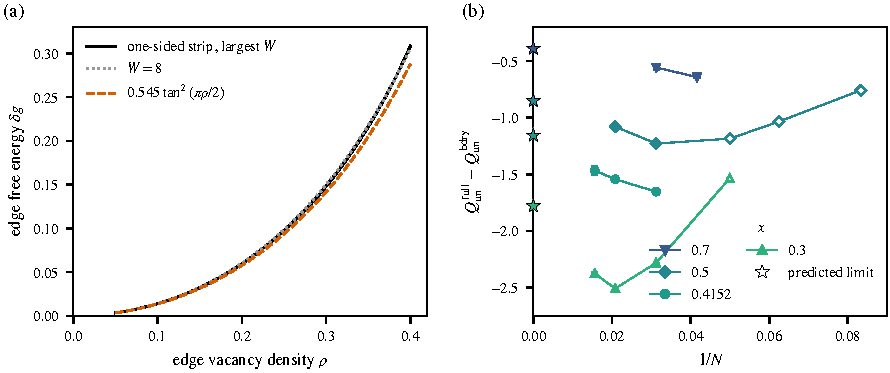
\includegraphics[width=0.86\textwidth]{fig7_full_model.pdf}
\caption{Vacancies on all cells change the uncompensated edge charge by a constant that is predicted from the free energy of the edge. (a) Free energy $\delta g$ gained per edge cell when adsorbed vacancies may leave the outermost cells, from one-sided strips of the largest available width ($10\le W\le16$, line) and of width $W=8$ (dotted), and the leading term of Eq.~\eqref{eq:dglead} (dashed). (b) Difference of the uncompensated edge charge between the full and the boundary model against $1/N$ at fixed $x$. Open symbols: exact; filled symbols: Monte Carlo, with errors from the scatter between independent runs (mostly smaller than the symbols). Stars at $1/N=0$: limits predicted by Eq.~\eqref{eq:Dinf}, which use no data from the diamond. Dotted lines join each predicted limit to the largest size as a guide to the eye; they are not fits.}
\label{fig:full}
\end{figure*}

%=====================================================================
\section{Discussion}\label{sec:discussion}
%=====================================================================

\paragraph*{Mechanism.} The arctic phenomenon is a consequence of charged boundaries. A staircase edge forces the maximal slope on the height field, and the frozen regions are where this slope persists into the interior. A vacancy adsorbed on the edge removes one unit of that boundary charge. The balance between the cost of a vacancy pair, $2\ln(1/z)$, and the entropy it releases, at most $N\ln2$, defines the single variable $x$. Below the threshold the edges are compensated except near the corners, and what remains of the boundary charge is the logarithmic amount of Eq.~\eqref{eq:Qun}. In the height description this entire process is the response of a field with stiffness $\pi/16$ to four point charges $x\ln2$.

\paragraph*{Fragility of arctic order.} The length $\Nst=2\log_2(1/z)$ is short. For $z=10^{-3}$ it is 20 lattice spacings, whereas the bulk screening length, which grows as the power $z^{-4/7}$, is about twice as large and exceeds $\Nst$ by an increasing factor at smaller $z$. A diamond much larger than $\Nst$ retains frozen corners of only $(4/\pi)\ln(1/z)\approx9$ cells. Boundary-induced order is thus far more sensitive to thermal defects than bulk correlations are, because the entropy available to a defect that relieves a frozen region grows with the size of the region.

\paragraph*{Neutral versus charged boundaries.} At a straight boundary the fugacity of boundary monomers does not change the macroscopic height~\cite{berestycki2023}. At a staircase boundary it sets the boundary slope and with it the limit shape. The distinction is the line charge of Sec.~\ref{sec:model}, and it applies to any bipartite dimer model: a boundary whose outermost sites belong to one sublattice is a charged plate.

\paragraph*{Artificial spin ice.} In vertex-frustrated artificial spin ices whose low-energy states are dimer covers~\cite{lao2018}, the excitations play the role of vacancies with $z=\ee^{-E_d/k_BT}$. Our results translate into two statements that can be tested on finite arrays with staircase-type boundaries: boundary-induced order should be visible only in arrays smaller than $\Nst=2E_d/(k_BT\ln2)$ lattice spacings, and in larger arrays ordered corners of size $(4/\pi)E_d/k_BT$ should remain, independent of the array size. These follow from Gauss's law for the emergent charge and from the stiffness of the height field, and do not depend on details of the dimer weights. We regard them as design guidelines; we have not modeled a specific array, the kinetics of its defects, or interactions between them.

\paragraph*{Range of validity.} The solution is derived from the variational principle of Eq.~\eqref{eq:var0}, which we support by an argument (Appendix~\ref{app:variational}) and by the enumeration, not by a proof. The agreement with enumeration is established for the boundary model at $0.1\le x\le0.9$ and $N\le192$. For the full model the equality of $\sig(x)$ rests on the locality argument of Sec.~\ref{sec:tests} and on the agreement of the predicted constants $D_\infty$ with Monte Carlo data at three values of $x$. The scaling limit requires $N$ to be smaller than the bulk screening length; for larger diamonds bulk vacancies are present, and we have not treated that regime. The frozen boundaries of Fig.~\ref{fig:frozen}(a) have been checked against the arctic circle at $x\to1$ only.

\paragraph*{Open problems.} Ciucu and Krattenthaler asked for the correlation of boundary dents in the generic case in which the segments joining them do not all cross the inscribed circle~\cite{ciucu2023}. The present solution answers a thermodynamic version of that question, with a number of dents proportional to $N$. A proof would require the two steps named in Sec.~\ref{sec:tests}. It would also be of interest to close Eqs.~\eqref{eq:xcond} and \eqref{eq:sigexact} in elliptic integrals, to obtain the edge free energy $\delta g(\rho)$ beyond its leading term and the $1/N$ approach seen in Fig.~\ref{fig:full}(b), and to treat regions with both neutral and charged edges.

%=====================================================================
\section{Conclusion}\label{sec:conclusion}
%=====================================================================

Thermal vacancies melt the arctic order of the Aztec diamond when the diamond is larger than $\Nst=2\log_2(1/z)$. The staircase edges are charged plates that adsorb vacancies, and in the scaling limit the fugacity acts on the height field only as point charges of strength $x\ln2$ at the four corners. The resulting free-boundary problem is solved by a hodograph transformation. Its solution gives, without adjustable parameters, the uncompensated edge charge, the vacancy profile, and frozen regions that have shrunk to corners whose size in a large diamond is $(4/\pi)\ln(1/z)$ lattice spacings. The solution agrees with exact enumeration of the boundary model to between $10^{-6}$ and $10^{-4}$.

\begin{acknowledgments}
This research was supported by the National Research Foundation (NRF) of Korea funded by the Korean Government (NRF-2023R1A2C1006050). Numerical codes and the text of the manuscript were prepared with the assistance of Claude (Anthropic). The author verified the results and is responsible for the content.
\end{acknowledgments}

\section*{Data availability}
The codes and data that support the findings of this article are openly available~\cite{repo}.

\appendix

%=====================================================================
\section{Boundary Pfaffian of the Aztec diamond}\label{app:pfaffian}
%=====================================================================

For a planar graph with monomers allowed only on its outer face the monomer-dimer partition function is a Pfaffian~\cite{giuliani2016}. For the Aztec diamond we use it in the following form. Label the $4N$ outermost cells $a=1,\dots,4N$ in cyclic order around the boundary, let $e_a\in\{0,1,2,3\}$ be the edge of cell $a$, and let $Z_0=2^{N(N+1)/2}$. Then
\begin{equation}\label{eq:pf}
  \left(\frac{Z}{Z_0}\right)^{2}=\det\left(1+z^2\,S\tilde G\right),\qquad S_{ab}={\rm sgn}(b-a),
\end{equation}
where $\tilde G_{ab}=(-1)^{e_a+e_b}\,{\rm sgn}(b-a)\,R(i,j)$ if $a$ and $b$ lie on adjacent edges and $\tilde G_{ab}=0$ otherwise. Here $i$ and $j$ are the positions of the two cells counted from the corner they share, starting from $0$, and
\begin{equation}
  R(i,j)=\sum_{k=0}^{N-1}\binom{k}{i}\binom{k}{j}\,2^{-k-1}
\end{equation}
is the ratio $M(A\setminus\{a,b\})/M(A)$ obtained by Ciucu and Krattenthaler~\cite{ciucu2023}. The magnitude of the entries is thus known; the signs in $\tilde G$ and $S$ are our convention for the cyclic labeling. We checked Eq.~\eqref{eq:pf} against a direct sum over all vacancy sets for $N=2$ and $3$ and against transfer-matrix enumeration for $N\le12$, and we have not derived the sign rule from Ref.~\cite{giuliani2016}. The mean number of vacancies is $z\,\partial\ln Z/\partial z$, and the density on a given cell follows from a cell-dependent fugacity.

%=====================================================================
\section{Solution in the hodograph plane}\label{app:rh}
%=====================================================================

Write $\lambda=\ii\mu$ with $\mu=(1-\zeta^2)/(1+\zeta^2)$. The center O of the diamond gives the particular solution $\Psi_0=1-\ii\mu$ of Eq.~\eqref{eq:burgers}, for which $u=v=1$. On the real side of the sector $\mu$ is real, so that $u=1$ on MO requires ${\rm Im}(\Psi-\Psi_0)=0$ and $v=0$ on the edge requires ${\rm Re}\,\Psi=0$; the conditions on the ray and on the arc follow from the reflection symmetries. In the variable $J=(\zeta^4+\zeta^{-4})/2$ the real side is the half line $J>1$, with M at $J_M=(\rM^4+\rM^{-4})/2$, and the remaining boundary is the half line $J<1$. The solution that is finite everywhere is
\begin{equation}
  \Psi=1-\ii\mu+\ee^{-\ii\pi/4}\sqrt{\mu}\,(1-J)^{1/4}(J_M-J)^{1/2}\,\Phi(J),
\end{equation}
\begin{equation}
  \Phi(J)=-\frac{2^{3/4}}{c_1}\,\frac{1}{\epsilon^{-1}-\epsilon}\sum_{n\ge0}a_n\epsilon^n ,
\end{equation}
with $c_0=(1+J_M)/2$, $c_1=(J_M-1)/2$, $\epsilon$ the root of $\epsilon+\epsilon^{-1}=2(c_0-J)/c_1$ with $|\epsilon|<1$, and $a_n$ the cosine coefficients of
\begin{equation}
  2\cosh\!\left[\tfrac14{\rm arccosh}(c_0-c_1\cos\varphi)\right]=\sum_{n\ge0}a_n\cos n\varphi .
\end{equation}
On the edge, $J=c_0-c_1\cos\varphi$, this gives $u(\varphi)=1+(r+r^{-1})\sum_na_n\sin n\varphi/[2\sqrt{c_1}\sin(\varphi/2)]$, and on the axis MO, $v=1-\sum_na_n\epsilon^n/(r+r^{-1})$. Summing the series leads to Eqs.~\eqref{eq:u} and \eqref{eq:v}. The two forms were implemented independently and agree to $10^{-8}$ in $x$, $\sig$, and $\dst$ for $0.1\le\rM\le0.9$; the series loses accuracy for $x\lesssim0.1$, and the numbers quoted in this paper are from the elliptic form. Equation~\eqref{eq:xcond} is equivalent to $x\ln2=\int_{\rm MO}\ln[(1+r)/(1-r)]\,\dd v$, the total current through the symmetry axis.

On the arc, $\zeta=\ee^{-\ii\phi}$ with $0<\phi<\pi/4$, $\Psi$ is real and $\lambda=-T$ with $T=\tan\phi$. The frozen boundary is the envelope of the lines $v+Tu=\Psi(T)$, namely $u=\Psi'(T)$ and $v=\Psi-T\Psi'$, completed by the reflection $u\leftrightarrow v$. For $x=0.999$ this curve satisfies $(u-1)^2+(v-1)^2=1$ to within $3\times10^{-4}$.

%=====================================================================
\section{Argument for the variational principle}\label{app:variational}
%=====================================================================

Equation~\eqref{eq:Z} for the boundary model is $Z=\sum_Vz^{|V|}M(A\setminus V)$ with $V$ a subset of the $4N$ outermost cells. (i) For fixed $V$ the region $A\setminus V$ is simply connected, and its boundary height, rescaled by $N$, is within $O(1/N)$ of the function determined by the density of $V$ along the edges. By Theorem~4.3 of Ref.~\cite{cohn2001}, $\ln M(A\setminus V)$ equals $N^2$ times the maximal entropy for that boundary function, up to $o(N^2)$, for all regions whose normalized boundary heights are close to it. (ii) The boundary functions are Lipschitz and form a compact set, which can be covered by finitely many neighborhoods to which (i) applies; this is the covering argument used in Ref.~\cite{cohn2001}. (iii) The number of sets $V$ is at most $2^{4N}$, which contributes $O(N)$ to $\ln Z$. Together these give Eq.~\eqref{eq:var0} with the maximum taken over boundary densities and, for each density, over heights in the interior. The step we have not verified in the literature is the continuity of the maximal entropy as a function of the boundary function, which (ii) requires. For the full model the argument is not available in this form, because interior vacancies make the height multivalued; the evidence there is the comparison of Sec.~\ref{sec:tests}.

%=====================================================================
\section{Bulk screening and straight edges}\label{app:bulk}
%=====================================================================

This appendix collects properties of the vacancy plasma away from charged boundaries. They are numerical checks of field-theory predictions and are not used in the solution of the diamond.

\paragraph*{Bulk.} A vacancy has scaling dimension $1/4$, so the fugacity is relevant with eigenvalue $7/4$. The vacancy density therefore scales as $n\propto z^{8/7}$ and the screening length as $\xi\propto z^{-4/7}$. The plasma maps onto the sine-Gordon model at $\beta^2=1/8$ (in the normalization in which the free-fermion point is $\beta^2=1/2$), for which $\xi_{\rm sG}=\beta^2/(1-\beta^2)=1/7$. Combining the exact free energy $f=-(M^2/4)\tan(\pi\xi_{\rm sG}/2)$~\cite{TODO-destri1991,TODO-zamolodchikov1995} with the mass $m_1=2M\sin(\pi\xi_{\rm sG}/2)$ of the lightest breather and $n=-z\,\partial f/\partial z$ gives the universal ratio
\begin{equation}
  \frac{m_1^2}{n}=7\sin\frac{\pi}{7}\approx3.037 ,
\end{equation}
where $m_1$ is the smallest inverse correlation length. Transfer matrices on cylinders give $3.041(9)$, which excludes the Debye-H\"uckel value $\pi$. Monte Carlo simulations of the bulk give a local exponent of $n(z)$ between $1.11$ and $1.16$ for $0.005\le z\le0.1$ and are consistent with perfect screening~\cite{TODO-stillinger1968}.

\paragraph*{Straight edge.} For a neutral edge the boundary scaling dimension of a charge-$q$ vacancy is $q^2/2$; transfer matrices on open strips of width 16 give $0.4986$ for $q=1$ and $1.962$ for $q=2$. This corresponds to an image charge of the same sign: within the screening length the vacancy density is depleted near the edge as $d^{1/4}$, and we measure exponents between $0.237$ and $0.258$. A separate fugacity $z_b$ for the edge cells is relevant with eigenvalue $1/2$ and drives a crossover to the opposite-sign image at a distance $\ell_b\approx0.3\,z_b^{-2}$, which is consistent with the convergence to a Neumann field proved for monomers on the boundary alone~\cite{berestycki2023} and with the two cases distinguished by Ciucu~\cite{ciucu2014}. At uniform small $z$ the screening length is much shorter than $\ell_b$, so the edge acts as a neutral boundary with a same-sign image.

\paragraph*{Staircase edge.} On strips bounded by staircase edges the charge adsorbed per edge cell converges to $(1-n)/2$, and the deviation of the charge density from its bulk value decays as $\ee^{-m_1d}$ with the distance $d$ from the edge.

%=====================================================================
\section{Numerical methods}\label{app:numerics}
%=====================================================================

\paragraph*{Transfer matrices.} The staircase strip of Sec.~\ref{sec:uniform} was solved with a transfer matrix acting on lattice diagonals, for $6\le W\le14$; the leading eigenvector was obtained with a sparse iterative solver, which does not converge for $z\lesssim2\times10^{-4}$, and those points are omitted from Fig.~\ref{fig:iso}(a). The lozenge capacitor was solved on rings of 12 and 16 cells with $16\le N\le64$ layers.

\paragraph*{Boundary enumeration.} The determinant in Eq.~\eqref{eq:pf} was evaluated with ball arithmetic at a working precision of $6N+400$ bits, with the matrix entries entered as exact rationals; the rigorous error radii are negligible. The mean density was obtained from a symmetric difference in $\ln z$ with relative step $10^{-30}$. The size $N=256$ exceeded the available memory.

\paragraph*{Sampling.} The configuration in Fig.~\ref{fig:model}(c) was generated in two steps. The vacancy set was sampled by a Metropolis algorithm on subsets of the outermost cells with weight $z^{|V|}M(A\setminus V)$, where $M$ is computed as a Kasteleyn determinant~\cite{TODO-kasteleyn1961}; the tiling was then drawn exactly, domino by domino, from the inverse Kasteleyn matrix. At $N=24$ and $x=0.5$ the sampled density profile agrees with the exact one within statistical error (mean number of vacancies per edge $4.06$ against $4.01$).

\paragraph*{Full model.} Exact results for $N\le20$ were obtained by transfer matrices. Larger sizes were simulated by Monte Carlo with local moves and parallel tempering in $z$, with 4 or 8 independent runs per size, half started from the frozen tiling and half from the empty lattice. Errors are the standard deviation of the run means divided by the square root of their number; with 4 runs this can underestimate the error. The code reproduces five exact values at $N=16$ and $20$ within one standard error. For $z\lesssim3\times10^{-5}$ at $N=64$ the two kinds of initial state do not meet within $4\times10^7$ sweeps, and such points are excluded.

\paragraph*{Software.} The codes were written with the assistance of an AI system (Claude, Anthropic). The core routines are covered by tests that compare independent implementations, including the closed-form boundary kernel against direct enumeration.

%=====================================================================
\section{Edge free energy from one-sided strips}\label{app:dg}
%=====================================================================

The function $\delta g(\rho)$ of Eq.~\eqref{eq:dg} is defined in the limit $z\to0$ at fixed edge density, in which no vacancy pair exists in the interior. A strip with vacancies allowed on all cells reaches this limit slowly, because at the widths accessible to transfer matrices the fugacity that gives $\rho\gtrsim0.35$ is not small. We therefore use a one-sided strip of width $W$: vacancies of the color of the left edge are allowed on every cell, and vacancies of the other color only on the outermost cells of the right edge. A neutral pair cannot form in the interior, and the limit is reached up to terms of order $\tan^W(\pi\rho/2)$. The reference is the same strip with vacancies on the outermost cells of both edges. The two are compared at equal density, through the Legendre transform $\phi(\rho)=\ln\Lambda(z)-2\rho\ln z$ of the logarithm of the largest eigenvalue $\Lambda$ of the transfer matrix, and $\delta g=\phi_{\rm one}-\phi_{\rm bdry}$; a comparison at equal $z$ would add a correction of order $1/W$ from the shift of the state. For $\rho=0.1$, $0.2$, $0.3$, and $0.4$ the widths $W=8$, $12$, and $16$ give $\delta g=0.014035$, $0.013946$, $0.013914$; $0.060152$, $0.059672$, $0.059501$; $0.149861$, $0.148686$, $0.148101$; and $0.305246$, $0.308423$, $0.308052$. The derivative in Eq.~\eqref{eq:Dinf} was taken by a symmetric difference with step $0.01$ in $x$; replacing the table for $W\le16$ by that for $W\le12$ changes $D_\infty$ by less than $0.005$.

\paragraph*{Leading term.} The strip has an exact description by walls. The cells with $X+Y=s$ form layers $s=0,\dots,2W-1$, each of one color. Without vacancies layers $2j$ and $2j+1$ are matched to each other, with all dominoes of the pair tilted the same way; a vacancy, or a domino that leaves the pair, is a wall between the two tilts. Three rules follow. Within a pair the walls of the two colors alternate along the strip, $\alpha_i<\beta_i<\alpha_{i+1}$, with no other constraint and unit weight. A wall of color $B$ in pair $j$ is a wall of color $A$ in pair $j+1$, displaced by one cell. A vacancy of color $A$ in layer $2j$ adds a wall to pair $j$, which the boundary model allows for $j=0$ only. The transfer operator across a pair is that of free fermions with symbol $(1+w)/(1-w)=\ii\cot(k/2)$; a wall crossing a pair has weight $1/\tan(\pi\rho/2)$, which is the origin of the suppression of interior vacancies.

For $\rho\to0$ the positions become continuous and the propagation to the far edge projects onto the ground state of the fermions, $\psi_n(x)=\prod_{i<j}|\sin\pi(x_i-x_j)/L|$ for $n$ walls on a strip of length $L$; here we take the width to infinity before the length. The vacancies on the edge of the boundary model are then distributed as the eigenvalues of the circular orthogonal ensemble, and the walls of the first pair as $\mu_n(x)\propto\psi_n(x)\prod_ig_i$, where $g_i$ are the gaps between neighbors. One wall created in the first pair instead of on the edge changes the weight by $\sum_i1/g_i$, while walls created deeper, or more than one of them, contribute at order $\rho^3$. Hence $\delta g=\kappa\rho^2+O(\rho^3)$ with $\kappa=\lim_{n\to\infty}\kappa_n$ and $\kappa_n=\langle n^{-1}\sum_i1/g_i\rangle_{\mu_n}L/n$. Since $\prod_ig_i$ is a Pfaffian and $\psi_n$ a determinant, $\kappa_n$ follows from de~Bruijn's integration formula. For even $n$ we find
\begin{equation}\label{eq:kappan}
  \kappa_n=1+\frac{2(n^2-1)}{3n}\biggl[\frac{\pi^2}{8}-\sum_{j=1}^{n/2}\frac{1}{(2j-1)^2}\biggr],
\end{equation}
so that $\kappa_n=4/3-(4/9)n^{-2}+\dots$ and $\kappa=4/3$. Equation~\eqref{eq:kappan} was identified from the exact values for $n\le14$ and agrees with the Pfaffian evaluation to 57 digits for all even $n\le40$; we have not proved it for general $n$. A Monte Carlo sampling of $\mu_n$ gives the same values. The transfer-matrix results for $\delta g/\rho^2$, extrapolated in the width as $W^{-2}$, are $1.362$, $1.387$, and $1.482$ at $\rho=0.06$, $0.10$, and $0.20$, and polynomial fits in $\rho$ give $1.341$ and $1.332$ at $\rho\to0$.

\bibliography{refs}
\end{document}
